%%%%%%%%%%%%%%%%%%%%%%%%%%%%%%%%%%%%%%%%%%%%%%%%%%%%%%%%%%%%%%%%%
%%% %
%%% % weiiszablon.tex
%%% % The Faculty of Electrical and Computer Engineering
%%% % Rzeszow University Of Technology diploma thesis Template
%%% % Szablon pracy dyplomowej Wydziału Elektrotechniki 
%%% % i Informatyki PRz
%%% % January, 2024
%%%%%%%%%%%%%%%%%%%%%%%%%%%%%%%%%%%%%%%%%%%%%%%%%%%%%%%%%%%%%%%%%

\documentclass[12pt,twoside]{article}

\usepackage{weiiszablon}

\author{Michał Bazan}

% np. EF-123456, EN-654321, ...
\studentID{EF-163881}

\title{Porównanie algorytmów nawigacyjnych}
\titleEN{Comparison of navigation algorithms}


%%% wybierz rodzaj pracy wpisując jeden z poniższych numerów: ...
% 1 = inżynierska	% BSc
% 2 = magisterska	% MSc
% 3 = doktorska		% PhD
% 4 = praca inżynierska
%%% na miejsce zera w linijce poniżej
\newcommand{\rodzajPracyNo}{2}


%%% promotor
\supervisor{dr inż. Dariusz Rzońca}
%% przykład: dr hab. inż. Józef Nowak, prof. PRz

%%% promotor ze stopniami naukowymi po angielsku
\supervisorEN{Dariusz Rzońca, dr. engineer}

\abstract{Praca koncentruje się na badaniu wybranych algorytmów nawigacyjnych oraz metod optymalizacji nastaw regulatorów PID z wykorzystaniem zbudowanego robota mobilnego, który został skonstruowany zgodnie z procedurami ASPICE. Celem jest ocena dokładności, szybkości wyznaczania trasy oraz ogólnej wydajności tych algorytmów. Analiza wyników pozwoli wyciągnąć wnioski dotyczące skuteczności i efektywności badanych algorytmów nawigacyjnych. Dzięki zastosowaniu standardów ASPICE zapewniona została wysoka jakość procesu budowy robota, co umożliwia rzetelne i wiarygodne badania nad jego funkcjonalnością i algorytmami nawigacyjnymi.}
\abstractEN{
The work focuses on the study of selected navigation algorithms and methods for optimising PID controller settings using a built mobile robot that has been constructed according to ASPICE procedures. The aim is to evaluate the accuracy, routing speed and overall performance of these algorithms. Analysis of the results will allow conclusions to be drawn regarding the effectiveness and efficiency of the navigation algorithms studied. Through the use of ASPICE standards, the high quality of the robot construction process is ensured, enabling reliable and credible research into its functionality and navigation algorithms.}

\keywords{Algorytmy nawigacyjne, Robot mobilny, Inżynieria, ASPICE, Machine Learning}
\keywordsEN{Navigation algorithms, Mobile robot, Engineering, ASPICE, Machine Learning}


\begin{document}

% strona tytułowa
\maketitle

\blankpage

% spis treści
\tableofcontents

\clearpage
\blankpage


\section*{Wykaz symboli, oznaczeń i skrótów}
\begin{enumerate}[label=\alph*), leftmargin=1.25cm]
	\item PID (eng. Proportional-Integral-Derivative) - skrót od Proporcjonalno-Całkująco-Różniczkującego regulatora, który jest powszechnie stosowany w systemach sterowania,
	\item MCU (eng. Microcontroller Unit) - Jednostka Mikrokontrolera,
	\item SQT (eng. Software Qualification Test) to proces testowania oprogramowania w celu zweryfikowania, czy spełnia ono określone wymagania i standardy jakościowe. SQT ma na celu potwierdzenie, że oprogramowanie działa zgodnie z założeniami i spełnia oczekiwania użytkowników oraz wymagania funkcjonalne i niefunkcjonalne.
\end{enumerate}

\section{Wstęp}
W dzisiejszych czasach, wraz z dynamicznym rozwojem technologii mobilnych, algorytmy nawigacyjne i uczenia maszynowego \cite{deepLearning} odgrywają kluczową rolę w różnorodnych aplikacjach, począwszy od systemów nawigacji w samochodach po autonomiczne roboty poruszające się w różnych środowiskach. Biorąc pod uwagę aktualność tych zagadnień i rosnące zapotrzebowanie, zdecydowano o przeprowadzeniu badań dotyczących systemów nawigacyjnych.
   
Celem tej pracy jest zbadanie heurystycznych metod \cite{genetics} optymalizazcji regulatorów PID oraz porównanie wybranych algorytmów pod kątem kryteriów takich jak dokładność wyznaczania trasy oraz wydajność obliczeniowa w różnych warunkach terenowych.  

Zakres pracy obejmuje dwie części:
\begin{enumerate}[label=\alph*), leftmargin=1.25cm]
	\item część inżynierska - wykonanie robota mobilnego, implementacja systemu wbudowanego oraz implementacja oprogramowania sterującego robotem poprzez dostępny interfejs,
	\item część badawcza - badanie algorytmów uczenia maszynowego do optymalizacji nastaw regulatorów PID oraz porównanie wybranych algorytmów nawigacyjnych. 
\end{enumerate}

Zastosowanie standardu ASPICE \cite{SPICE} zapewnia wysoką jakość procesu budowy robota oraz implementacji oprogramowania co pozwola na przeprowadzenie rzetelnych badań i wyciągnięcie wiarygodnych wniosków.

W dalszej części pracy szczegółowo omówione zostaną poszczególne etapy realizacji każdego z tych komponentów, prezentując zarówno teoretyczne założenia, jak i praktyczne wyniki osiągnięte w ramach projektu.

W następnych rozdziałach pracy przedstawiono szczegółowy opis inżynierskiej części projektu oraz wyniki przeprowadzonych badań. W rozdziale poświęconym inżynierskiej części projektu omówiono budowę robota, jego system operacyjny oraz prostą stację operatorską, które stanowią podstawę do realizacji badań algorytmicznych. Następnie, w rozdziale dotyczącym badanych algorytmów, zaprezentowano teoretyczne i praktyczne aspekty algorytmu genetycznego, algorytmów nawigacyjnych statycznych oraz dynamicznych. Kolejny rozdział skupia się na opisie przeprowadzonych badań, w których dokonano optymalizacji nastaw regulatora PID oraz przeprowadzono porównanie skuteczności algorytmów nawigacyjnych. Te szczegółowe analizy mają na celu ocenę wydajności poszczególnych rozwiązań oraz identyfikację optymalnych metod nawigacyjnych dla zbudowanego robota.

\section{Inżynierska część projektu}

W tym rozdziale przedstawiono kompleksowy opis prac związanych z implementacją oraz funkcjonowaniem robota. Niniejszy rozdział stanowi szczegółowe omówienie trzech kluczowych elementów projektu, które skupiały się na budowie fizycznej robota zgodnie z procedurami SPICE, implementacji oprogramowania w języku C++ z uwzględnieniem unit testów oraz oprogramowania do sterowania robotem. Dzięki zastosowaniu tych trzech elementów możliwe było zapewnienie nie tylko skutecznej implementacji samego robota, ale również jego oprogramowania oraz efektywnego zarządzania nim w czasie rzeczywistym.
Dokładna dokumentacja wszystkich komponentów projektu oraz testów znajduje się na repozytorium Github \cite{repo}.

\subsection{Budowa robota}

Pierwszym aspektem, który został przedstawiony, jest proces budowy robota. Opisane zostały tutaj szczegóły dotyczące wyboru komponentów oraz implementacji elektroniki sterującej. Proces ten obejmuje kilka kluczowych etapów, które mają na celu zapewnienie, że robot będzie w stanie spełniać wszystkie założone funkcje i wymagania. W szczególności skupiono się na doborze odpowiednich czujników, kontrolerów, silników oraz systemu zasilania, które umożliwią robotowi prawidłowe działanie w różnych warunkach.

\subsubsection{Wymagania sprzętowe}

W celu dobrania właściwych elementów do budowy robota, sformułowano niżej umieszczone wymagania wysokiego poziomu. Te wymagania określają kluczowe funkcje i cechy, jakie powinny posiadać komponenty sprzętowe robota, aby zapewnić jego pełną funkcjonalność i niezawodność. W tabeli \ref{Tab:HWE1} zestawiono najważniejsze z tych wymagań, które dotyczą obsługi czujników, komunikacji bezprzewodowej, napędu oraz zarządzania zasilaniem.

\begin{table}[ht]
\caption{Wymagania wysokiego poziomu HWE1}
\centering		
	\begin{tabular}{|c|p{0.7\textwidth}|}	
		\hline
		ID\_HWE1 & Opis \\
		\hline
		HWE\_1\_010 & Sprzęt powinien wspierać obsługę czujników odległości. \\
		\hline
		HWE\_1\_020 & Kontroler powinien udostępniać moduł WiFi. \\
		\hline 
		HWE\_1\_030 & Robot powinien być wyposażony w szczotkowe silniki DC z enkoderami.\\
		\hline
		HWE\_1\_040 & Sprzęt powinien wspierać obsługę enkoderów. \\
		\hline
		HWE\_1\_060 & Sprzęt powinien mieć zaimplementowany odpowiedni system dystrybucji zasilania. \\
		\hline

	\end{tabular}	
	
\label{Tab:HWE1}
\end{table}	

\newpage

Na podstawie wyżej ukazanych wymagań wysokiego poziomu, sformułowano następujące wymagania niskiego poziomu. Te szczegółowe wymagania określają dokładne specyfikacje techniczne i parametry, które muszą być spełnione przez komponenty, aby zapewnić zgodność z ogólnymi celami projektu. W tabeli \ref{Tab:HWE2} zestawiono kluczowe wymagania dotyczące interfejsów komunikacyjnych, zasilania oraz czujników.


\begin{table}[ht]
\caption{Wymagania niskiego poziomu HWE2}
\centering
\begin{tabular}{|c|p{0.7\textwidth}|}	
    \hline
    ID\_HWE2 & Opis \\
    \hline
    HWE\_2\_010 & Wszystkie interfejsy komunikacyjne powinny wspierać logikę 3V3. \\
    \hline
    HWE\_2\_020 & Mikrokontroler powinien być wyposażony w moduł WiFi. \\
    \hline 
    HWE\_2\_030 & System dystrybucji zasilania powinien zasilić logikę.\\
    \hline
    HWE\_2\_040 & System dystrybucji zasilania powinien zasilić silniki. \\
    \hline
    HWE\_2\_060 & Czujnik odległości powinien mieć zakres pomiarowy wynoszący conajmniej 200 cm. \\
    \hline
    HWE\_2\_070 & Czujniki odległości powinny udostępniać interfejs komunikacyjny kompatybilny z interfejsami mikrokontrolera. \\
    \hline
\end{tabular}
\label{Tab:HWE2}
\end{table}
	

\begin{figure}[ht]%
 \centering%
 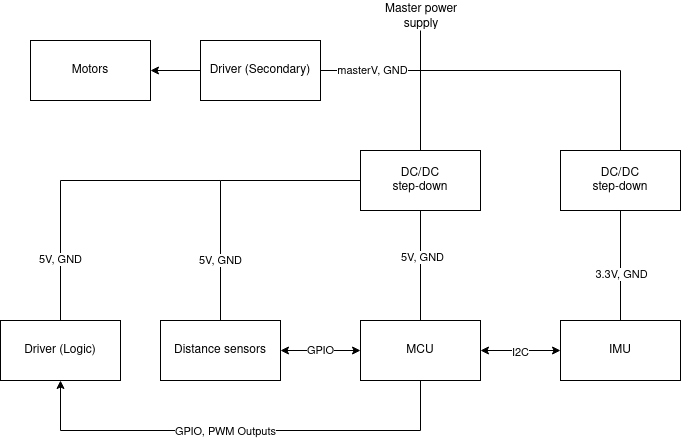
\includegraphics[width=12cm]{figures/engHW/robotblock.png}%
 \caption{Schemat blokowy sprzętu}%
 \label{Fig:schemat}%
\end{figure}

Niżej umieszczona figura \ref{Fig:schemat} ukazuje schemat blokowy utworzony na podstawie wcześniej zdefiniowanych wymagań sprzętowych. Wskazuje, jakie interfejsy i poziomy napięć zasilania zostały wykorzystane pomiędzy poszczególnymi blokami. Sprzęt zdefiniowany w ten sposób oraz zbiór wymagań stawianych przed urządzeniem umożliwił dobór właściwych komponentów.

\newpage

\subsubsection{Schemat elektryczny}
Niniejsza sekcja skupia się na wyjaśnieniu schematu elektrycznego robota. 
Na podstawie umieszczonych w poprzedniej sekcji wymagań dokonano wyboru komponentów, które zostały wykorzystane w projekcie, ale dokładny opis elementów został umieszczony w dokumentacji tej części projektu na repozytorium Github \cite{repo}.\\
\newline
W celu ułatwienia procesu implementacji i zmitygowaniu potencjalnych błędów, schemat elektryczny został podzielony na bloki zgodnie z podziałem ukazanym na rysunku \ref{Fig:schemat}.



\begin{figure}[ht]%
 \centering%
 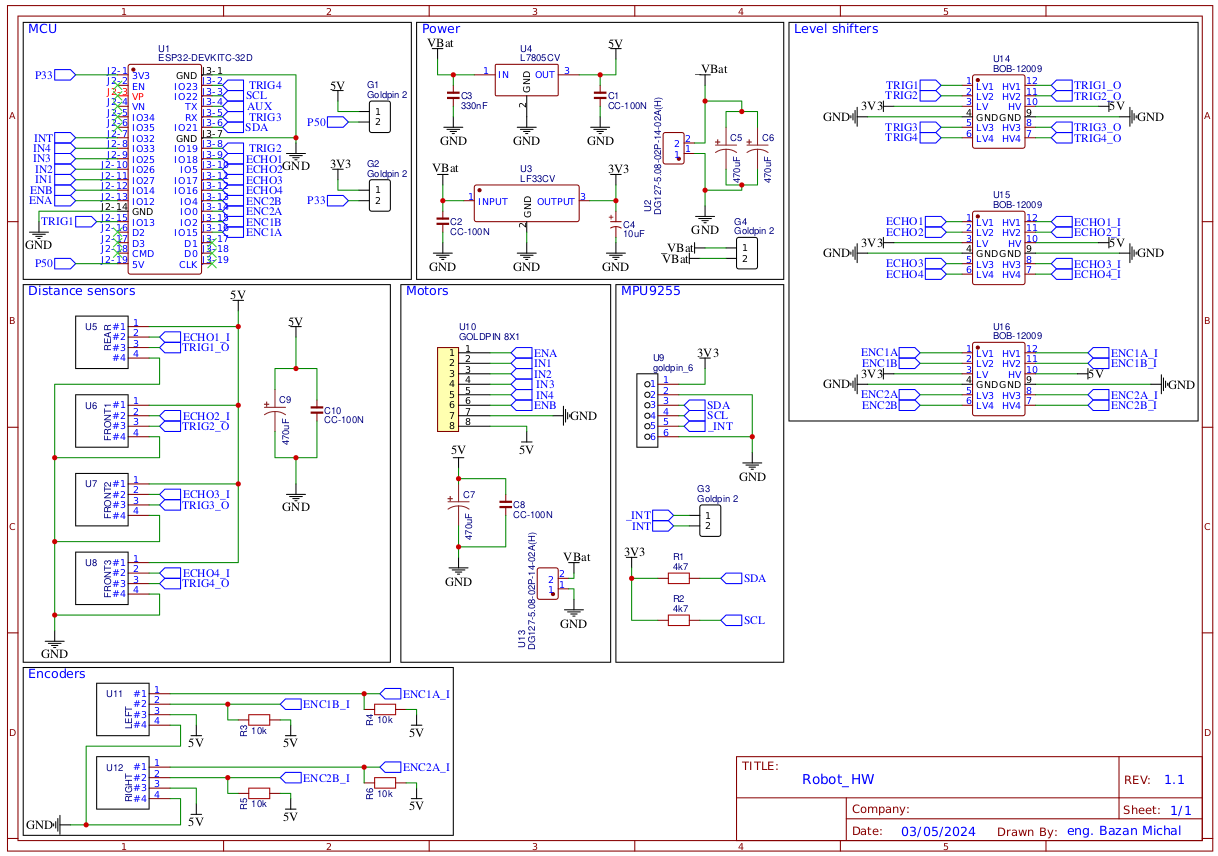
\includegraphics[width=12cm]{figures/engHW/robotschem.png}%
 \caption{Schemat elektryczny}%
 \label{Fig:elektryczny}%
\end{figure}

Wyżej umieszczona ilustracja \ref{Fig:elektryczny} ukazuje połączenia pomiędzy blokami schematu:

\begin{enumerate}[label=\alph*), leftmargin=1.25cm]
	\item MCU - blok definiuje wejścia i wyjścia sterujące oraz połączenia interfejsów komunikacyjnych,
	\item Power - sekcja odpowiedzialna za dystrybucję zasilania,
	\item Level shifters - konwertery poziomów logicznych, które zapewniają kompatybilność poziomów sygnałów elektrycznych,
	\item Distance sensors - blok definiuje połączenia pomiędzy mikrokontrolerem i czujnikami odległości,
	\item Motors - sekcja ukazuje sygnały sterujące silnikami,
	\item MPU9255 - blok został zaimplementowany, ale nie jest wykorzystywany,
	\item Encoders - ta sekcja ukazuje sygnały wyjściowe z enkoderów.
\end{enumerate}

\subsubsection{Testy}
Testowanie tej części projektu polegało głównie na weryfikacji założeń i projektu płytki, dlatego aspekt ten nie został poruszony w tej sekcji. Szczegółowa dokumentacja znajduje się w zdalnym repozytorium \cite{repo}. Testy obejmowały sprawdzenie zgodności z wymaganiami, poprawność połączeń oraz funkcjonalność poszczególnych bloków.

\newpage

\subsection{System operacyjny robota}

Ta sekcja skupia się na implementacji oprogramowania w języku C++, obejmującej zarówno projektowanie, jak i implementację funkcjonalności. System operacyjny robota zarządza wszystkimi aspektami operacyjnymi robota, od odczytu danych z czujników, poprzez przetwarzanie i analizę tych danych, aż po sterowanie silnikami i komunikację zewnętrzną.

\subsubsection{Wymagania dotyczące oprogramowania}

Na podstawie wcześniej omówionych wymagań sprzętowych oraz celów tego projektu, sformułowano następujące wymagania wysokiego poziomu. Wymagania te definiują kluczowe funkcjonalności, jakie powinno posiadać oprogramowanie, aby zapewnić niezawodność działania robota.

\begin{table}[ht]
\caption{Wymagania wysokiego poziomu SWE2}
\centering		
	\begin{tabular}{|c|p{0.7\textwidth}|}	
		\hline
		ID\_SWE2 & Opis \\
		\hline
		SWE\_2\_010 & Oprogramowanie powinno odczytywać sensory periodycznie. \\
		\hline
		SWE\_2\_020 & Interfejs WiFi powinien być wykorzystany do komunikacji z oprogramowaniem sterującym. \\
		\hline 
		SWE\_2\_030 & Oprogramowanie powinno udostępniać interfejs do sterowania silnikami.\\
		\hline
		SWE\_2\_040 & Komunikacja powinna wykorzystywać prosty protokół komunikacyjny do wymiany danych pomiędzy robotem a oprogramowaniem sterującym. \\
		\hline
		SWE\_2\_050 & Oprogramowanie powinno implementować algorytm wyznaczający odometrię. \\
		\hline

	\end{tabular}	
	
\label{Tab:SWE2}
\end{table}	

W celu wyłonienia konkretnych bloków, z jakich powinno składać się oprogramowanie, zdefiniowano następujące wymagania niskiego poziomu. Te szczegółowe wymagania określają specyficzne zadania i interfejsy, które muszą być zaimplementowane, aby spełnić wymagania wysokiego poziomu.

\begin{table}[ht]
\caption{Wymagania niskiego poziomu SWE3}
\centering		
	\begin{tabular}{|c|p{0.7\textwidth}|}	
		\hline
		ID\_SWE3 & Opis \\
		\hline
		SWE\_3\_010 & Oprogramowanie powinno odczytywać sensory co 50ms. \\
		\hline
		SWE\_3\_020 & Oprogramowanie powinno udostępniać interfejs do wymiany danych. \\
		\hline 
		SWE\_3\_030 & Oprogramowanie powinno udostępniać dane z sensorów na żądanie.\\
		\hline
		SWE\_3\_040 & Komunikacja powinna opierać się o wykorzystanie protokołu MQTT. \\
		\hline
		SWE\_3\_050 & Oprogramowanie powinno udostępnić interfejs do sterowania silnikami. \\
		\hline
		SWE\_3\_060 & Implementacja powinna wykorzystywać prostą odometrię. \\
				\hline
	\end{tabular}	
	
\label{Tab:SWE3}
\end{table}	

\newpage

Na podstawie wymagań umieszczonych w tabeli \ref{Tab:SWE3} zdefiniowano niżej ukazaną architekturę systemu operacyjnego robota. 

\begin{figure}[ht]%
 \centering%
 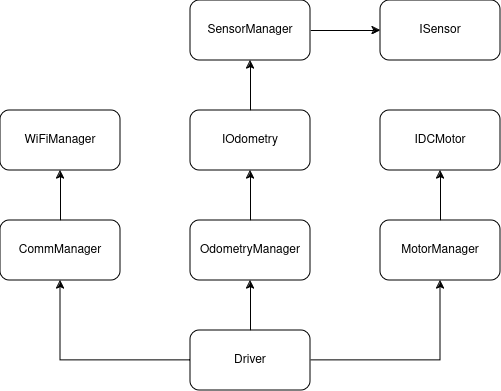
\includegraphics[width=12cm]{figures/engSW/block.png}%
 \caption{Architektura oprogramowania}%
 \label{Fig:architektura}%
\end{figure}

Na rysunku \ref{Fig:architektura} przedstawiono architekturę systemu operacyjnego robota, która została zaprojektowana w oparciu o zdefiniowane wymagania niskiego poziomu. Architektura ta składa się z kilku kluczowych modułów:

\begin{enumerate}[label=\alph*), leftmargin=1.25cm]
	\item CommManager - odpowiada za połączenie sieciowe i komunikację za pośrednictwem protokołu MQTT,
	\item SensorManager - posiada uchwyt do wszystkich dostępnych sensorów, które obsługuje periodycznie,
	\item OdometryManager - posiada uchwyt do obiektu typu SensorManager i realizuje odometrię na podstawie odczytów z czujników,
	\item MotorManager - steruje silnikami zależnie od nadchodzących komunikatów,
	\item Driver - odpowiada za poprawną inicjalizację systemu, wywoływanie funkcji callbackowych z bloku odpowiedzialnego za komunikację oraz ustawienie prędkości obrotowej silników zależnie od uchybu regulacji.  
\end{enumerate}

\subsubsection{Implementacja}
Implementacja systemu operacyjnego robota składa się z 12 klas, z których każda pełni określoną rolę w funkcjonowaniu robota. Klasy te są odpowiedzialne za zarządzanie różnymi aspektami operacyjnymi, od odczytu danych z czujników po sterowanie silnikami. Jednym z ważnych elementów implementacji jest także zaimplementowany prosty szablon regulatora PID oraz stos oparty o std::array\cite{stdarray}.

\begin{lstlisting}[language=C++, caption={Klasa CommManager}, label={lst:CommManager}]
template<class StringType, std::size_t topic_num>
class CommManager{
public:
    using messageType = std::tuple<StringType, StringType>;
    using onMsg_cb = std::function<void(char*, byte*, unsigned int)>;

    static messageType createMessage(const StringType& topic, const StringType& payload) noexcept;

    CommManager(
        WiFiManager<StringType>&& w, 
        const StringType& uname, 
        const StringType& broker, 
        const StringType& password, 
        WiFiClient& c, 
        std::array<StringType, topic_num>&& topics,
        const onMsg_cb& cback,
        const StringType& ID = "Robot"
        ) noexcept;

    MQTTStatus poolCommManager() noexcept;
    
    bool sendMessage(messageType&& message) noexcept;

private:
    NetworkStatus poolNetwork() noexcept;
    SemaphoreHandle_t MQTTQueueMutex;

    enum : uint8_t{
        ConnectingNetwork = 0,
        ConnectingBroker,
        Timeout,
        CheckingStatus
    };
    uint8_t m_internalState;
    WiFiManager<StringType> m_wifiMgr;
    custom::stack<messageType, stack_depth> m_messageStack;
    StringType m_broker;
    StringType m_password;
    StringType m_uname;
    StringType m_ID;
    const std::array<StringType, topic_num> m_topics;
    PubSubClient m_mqttClient;
    onMsg_cb m_message_cb;
};
\end{lstlisting}

Klasa CommManager (Listing \ref{lst:CommManager}) zarządza komunikacją między robotem a oprogramowaniem sterującym poprzez protokół MQTT i połączenie WiFi. Oferuje funkcje odczytu danych z czujników, wysyłania komunikatów i reakcji na przychodzące komunikaty. Metoda createMessage tworzy nową wiadomość MQTT na podstawie tematu i treści. W konstruktorze inicjalizowane są połączenie WiFi, parametry MQTT i lista subskrybowanych tematów. poolCommManager zarządza połączeniem z WiFi i brokerem MQTT, podejmując odpowiednie działania w zależności od stanu połączenia. sendMessage dodaje wiadomość do kolejki komunikatów. Klasa zapewnia niezawodne połączenie i efektywną komunikację, co jest kluczowe dla funkcjonowania robota w różnych scenariuszach działania.

\begin{lstlisting}[language=C++, caption={Klasa SensorManager}, label={lst:SensorManager}]
enum class SensorMapping : uint8_t{ 
    LEFT_Encoder,
    RIGHT_Encoder,
    DST_Front_1,
    DST_Front_2,
    DST_Front_3,
    DST_Rear
};

constexpr uint8_t translate(SensorMapping s){
    return static_cast<uint8_t>(s);
}

class SensorManager{
public:
    void init();
    SensorManager(std::array<sensorPointer, numSensors>&& s);
    void poolSensors();
    ISensor& getSensor(SensorMapping s);

private:
    std::array<sensorPointer, numSensors> sensors;
};
\end{lstlisting}

Klasa SensorManager (Listing \ref{lst:SensorManager}) zarządza sensorami robota, przechowując ich wskaźniki i udostępniając interfejs odczytu danych. Typ SensorMapping reprezentuje indeksy sensorów, ułatwiając dostęp do nich. Metoda translate przekształca enum na liczby całkowite, co umożliwia łatwiejszy dostęp do konkretnego urządzenia. Konstruktor inicjuje obiekt, a init inicjuje sensory. poolSensors odpytuje sensory, a getSensor zwraca referencję do konkretnego sensora.

\newpage

\begin{lstlisting}[language=C++, caption={Klasa OdometryManager}, label={lst:OdometryManager}]
enum ActiveOdometry : std::size_t {
    SimpleOdo = 0,
    AdvancedOdo = 1
};

constexpr std::size_t availableAlgorithms = 2;

class OdometryManager{
public:
    OdometryManager(
        std::array<IOdometry*, availableAlgorithms>&& odo,
        SensorManager& s
    ) noexcept;

    void updatePosition() noexcept;
    void setActiveOdometry(ActiveOdometry o) noexcept;
    std::size_t getActiveOdometry() const noexcept;
    const position getPosition() const noexcept;
    void resetActiveOdometry() noexcept;
private:
    std::array<IOdometry*, availableAlgorithms> m_odometryAgents;
    SensorManager& m_sensorMgr;
    std::size_t m_active;
};
\end{lstlisting}

Klasa OdometryManager zarządza różnymi algorytmami odometrii robota i aktualizuje jego pozycję na podstawie danych z sensorów. Enum ActiveOdometry definiuje dostępne algorytmy odometrii, lecz w tej implementacji dostępna jest tylko prosta odometria. Konstruktor przyjmuje tablicę wskaźników do obiektów IOdometry reprezentujących różne algorytmy odometrii oraz referencję do obiektu SensorManager. Metoda updatePosition aktualizuje pozycję robota na podstawie danych z sensorów i aktywnego algorytmu odometrii. setActiveOdometry ustawia aktywny algorytm odometrii, getActiveOdometry zwraca jego indeks, a getPosition zwraca aktualną pozycję. Metoda resetActiveOdometry resetuje aktywny algorytm i ustawia zerowe współrzędne. Klasa zapewnia elastyczne zarządzanie algorytmem odometrii i precyzyjne poruszanie się robota.


\begin{lstlisting}[language=C++, caption={Klasa MotorManager}, label={lst:MotorManager}]
class MotorManager{
public:
    enum class settingType{
        setAngularTarget,
        updatePwm
    };

    using motor_array = std::array<IDCMotor*, motor_num>;
    using speed_array = std::array<int32_t, motor_num>; 
    using angular_array = std::array<float, motor_num>;

    void init() noexcept;
    void setSpeed(const speed_array& speeds, settingType t = settingType::updatePwm) noexcept;
    MotorManager(motor_array&& m, float i = inertia_coef) noexcept;
    void InertiaCoef(float i) noexcept;
    float InertiaCoef() const noexcept;
    void poolMotors() noexcept;
    const speed_array* CurrentSpeed() const noexcept;
    const speed_array* DesiredSpeed() const noexcept;
    const angular_array* TargetAngular() const noexcept;

private:
    float m_inertiaCoef;
    motor_array motors;
    speed_array target_percent_speed;
    speed_array current_percent_speed;
    angular_array target_angular_speed;
};
\end{lstlisting}

Klasa MotorManager zarządza silnikami prądu stałego robota, kontrolując ich prędkość obrotową i kierunek. settingType definiuje różne typy ustawień silników, a motor\_array, speed\_array, i angular\_array to odpowiednio tablice wskaźników do silników, prędkości silników i prędkości kątowych. Metoda init inicjuje silniki, setSpeed ustawia prędkość zależnie od typu ustawienia, a konstruktor inicjuje obiekt, przyjmując tablicę wskaźników do silników i opcjonalny współczynnik inercji. poolMotors aktualizuje stany silników, a CurrentSpeed, DesiredSpeed, i TargetAngular zwracają odpowiednio aktualną prędkość, docelową prędkość i prędkości kątowe silników. Klasa zapewnia elastyczne zarządzanie silnikami i kontrolę nad ich prędkościami, kluczową dla ruchu i sterowania robotem.

\begin{lstlisting}[language=C++, caption={Klasa Kernel}, label={lst:Kernel}]
class Kernel{
public:
    static void init();
    static void main();
    
    /* motion management */
    static Motor::DCMotor motorLeft;
    static Motor::DCMotor motorRight;
    static Motor::MotorManager motorManager;
    static uint32_t mapper(uint32_t);
    static constants::motors::types::motor_pid pidLeft;
    static constants::motors::types::motor_pid pidRight;

    /* communications management */
    static constants::comm::types::job_stack_t jobStack;
    static Comm::MQTT::CommManager<String, constants::comm::subscribedTopics> commMgr;
    static void MQTTcallback(char*, byte*, unsigned int);

    /* sensor management */
    static Sensor::DistanceSensor rear;
    static Sensor::DistanceSensor front_left;
    static Sensor::DistanceSensor front;
    static Sensor::DistanceSensor front_right;
    static Sensor::Encoder encoderLeft;
    static Sensor::Encoder encoderRight;

    static Sensor::SensorManager sensorMgr;

    static Sensor::simpleOdometry odoAgent;
    static Sensor::OdometryManager odoMgr;
};    
\end{lstlisting}

Klasa Kernel pełni kluczową rolę jako centralny moduł zarządzający systemem. Odpowiada za inicjalizację systemu oraz koordynację jego głównych funkcji. Metoda init przygotowuje system do działania, a main zarządza jego główną logiką. Kluczowe funkcje obejmują zarządzanie ruchem (silniki, regulator PID), komunikacją (MQTT), sensorami (odległości, enkodery) oraz odometrią. Kernel integruje te komponenty, zapewniając ich współpracę i efektywną działalność.

\subsubsection{Obsługiwane polecenia}

Sekcja przedstawia interfejs sieciowej komunikacji z robotem poprzez protokół MQTT. Tabela \ref{Tab:RobotSub} zawiera tematy subskrybowane przez robota wraz z opisem ich przeznaczenia oraz przykładowymi danymi. Tabela ta obejmuje kanały do debugowania, przesyłania komend oraz ustawiania prędkości silników. Natomiast w tabeli \ref{Tab:RobotPub} znajdują się tematy publikowane przez robota, wraz z opisem i typowymi danymi przesyłanymi przez te kanały, takimi jak odpowiedzi na komendy i wiadomości debugujące. W tabeli \ref{Tab:RobotCMD} znajdują się dostępne komendy, ich opisy oraz oczekiwane odpowiedzi. Komendy obejmują pobieranie odczytów z czujników, resetowanie pozycji, pobieranie danych odometrycznych oraz zatrzymywanie silników.

\begin{table}[ht]
\caption{Tematy subskrybowane przez robota}
\centering		
	\begin{tabular}{|p{0.2\textwidth}|p{0.4\textwidth}|p{0.3\textwidth}|}	
		\hline
		Robot subskrybuje & Opis & Dane \\
		\hline
		robot/echo/in & Temat wykorzystywany do debugu, system odpowiada ciągiem tekstowym na temacie robot/echo/out. & Dowolny ciąg tekstowy zgodny z ASCII. \\
		\hline
		robot/cmd/in & Temat do przesyłania zdefiniowanych komend (tab. \ref{Tab:RobotCMD} ). & Komenda jako ciąg tekstowy zgodny z ASCII. \\
		\hline
		robot/set/motors & Temat do przesyłania żądanych prędkości silników. & Dane w formacie JSON: \{ „left” : x, „right” : y \}, gdzie x oraz y to prędkości wyrażone w procentach. \\
		\hline
	\end{tabular}	
	
\label{Tab:RobotSub}
\end{table}	

\begin{table}[ht]
\caption{Tematy publikowane przez robota}
\centering		
	\begin{tabular}{|p{0.2\textwidth}|p{0.4\textwidth}|p{0.3\textwidth}|}	
		\hline
		Robot subskrybuje & Opis & Dane \\
		\hline
		robot/echo/out & Temat, na który system przesyła wiadomości dotyczące debugu. & Dowolny ciąg tekstowy zgodny z ASCII. \\
		\hline
		robot/cmd/response & Odpowiedź na przesłaną komendę. & Dane w formacie JSON (odczyty z sensorów, odometria), brak odpowiedzi lub ciąg tekstowy "cmd not supported" w przypadku przesłania błędnej komendy. \\
		\hline
	\end{tabular}	
	
\label{Tab:RobotPub}
\end{table}	

\begin{table}[ht]
\caption{Dostępne komendy}
\centering		
	\begin{tabular}{|p{0.2\textwidth}|p{0.4\textwidth}|p{0.3\textwidth}|}	
		\hline
		Komenda & Opis & Odpowiedź \\
		\hline
		get\_sensors & Pobierz odczyty z czujników. & Dane z czujników w formacie JSON. \\
		\hline
		reset\_odo & Zeruj pozycję. & Brak odpowiedzi. \\
		\hline
		get\_odo & Pobierz wyznaczone dane odometryczne. & Dane w formacie JSON. \\
		\hline
		get\_all & Pobierz dane z sensorów i pozycję robota. & Dane w formacie JSON. \\
		\hline
		halt & Zatrzymaj silniki. & Brak odpowiedzi. \\
		\hline
	\end{tabular}	
	
\label{Tab:RobotCMD}
\end{table}	

\newpage
\subsubsection{Testy oprogramowania}
W tej sekcji opisano przeprowadzone testy weryfikujące zgodność oprogramowania z wymaganiami określonymi w specyfikacji SWE3.

\begin{table}[ht]
\caption{Test SQT\_01}
\centering		
	\begin{tabular}{|p{0.2\textwidth}|p{0.4\textwidth}|p{0.3\textwidth}|}	
		\hline
		Treść wymagania & Weryfikacja & Wynik testu \\
		\hline
		Oprogramowanie powinno odczytywać sensory co 50ms. & Zadanie odczytywania sensorów jest zaplanowane w systemie freeRTOS co 50ms. & Wynik pozytywny \\
		\hline
	\end{tabular}	
	
\label{Tab:TEST1}
\end{table}	

\begin{table}[ht]
\caption{Test SQT\_02}
\centering		
	\begin{tabular}{|p{0.3\textwidth}|p{0.3\textwidth}|p{0.3\textwidth}|}	
		\hline
		Weryfikacja & Oczekiwane & Obserwacja \\
		\hline
		Podłączenie płytki do zasilania &
		Płytka powinna być poprawnie zasilona &
		Płytka została poprawnie zasilona \\
		\hline
		Wgranie najnowszej wersji oprogramowania na płytkę &
		Najnowsze oprogramowanie powinno zostać wgranę na płytkę &
		Najnowsze oprogramowanie zostało wgrane na płytkę \\
		\hline
		Oczekiwanie na wiadomość "robot initialized" na temacie robot/echo/out. &
		Wiadomość powinna zostać odebrana. &
		Wiadomość została odebrana. \\
		\hline
		Przesłanie wiadomości na temacie robot/set/motors, aby ustawić prędkość silników bliską 40\% prędkości maksymalnej. 			&
		Silniki powinny kręcić się z prędkością bliską 40\% prędkości maksymalnej. &
		Silniki kręcą się z prędkością bliską 40\% prędkości maksymalnej. \\
		\hline
		Przesłanie komendy halt na temacie robot/cmd/in. &
		Silniki powinny się zatrzymać. &
		Silniki zatrzymały się. \\
		\hline
		Przesłanie komendy get\_all w celu uzyskania wszystkich danych. &
		Uzyskano dane z sensorów i pozycję robota. &
		Uzyskano dane z sensorów i pozycję robota. \\
		\hline
		Przesłanie komendy reset\_odo w celu resetowania odometrii. &
		Wiadomość powinna zostać wysłana. &
		Wiadomość została wysłana. \\
		\hline
		Przesłanie komendy get\_odo w celu uzyskania pozycji robota. &
		Uzyskano pozycję, która wskazuje na zero. &
		Uzyskano pozycję, która wskazuje na zero. \\
		\hline
	\end{tabular}	
	
\label{Tab:TEST1}
\end{table}	
\newpage

Test SQT\_01 miał na celu potwierdzenie, czy oprogramowanie regularnie odczytuje dane z czujników odległości co 50 ms, zgodnie z wymaganiami. Mimo że w projekcie nie wykorzystano IMU, to test został dostosowany do odczytu danych z czujników odległości, a zadanie zostało zaplanowane jako praca freeRTOS z interwałem 50 ms.

Testy oznaczone jako SQT\_02SWE, skupiły się na weryfikacji podstawowych funkcji oprogramowania, w tym dostarczania zasilania i programowania sprzętu, wymiany danych, kontroli silników itp. Każde z tych wymagań zostało poddane testowi, a wynikiem było potwierdzenie, że oprogramowanie spełnia te kryteria.

W obu przypadkach testy zakończyły się sukcesem, co potwierdza zgodność oprogramowania z wymaganiami określonymi w specyfikacji SWE3. Oprócz przeprowadzenia testów kwalifikacyjnych, oprogramowanie zostało pokryte testami jednostkowymi.

\section{Badane algorytmy}

\subsection{Algorytm genetyczny}
\subsection{Uczenie ze wzmocnieniem}
\subsection{Algorytmy nawigacyjne}


\section{Badania}
\subsection{Optymalizacja nastaw regulatora PID prędkości obrotowej}
\subsection{Optymalizacja nastaw regulatora położenia i orientacji}
\subsection{Porównanie algorytmów nawigacyjnych w terenie bez przeszkód}
\subsection{Porównanie algorytmów nawigacyjnych w terenie z przeszkodami}

\section{Podsumowanie i wnioski końcowe}


\section*{Załączniki}



\clearpage

\addcontentsline{toc}{section}{Literatura}

\begin{thebibliography}{6}
\bibitem{repo} https://github.com/DevxMike/master\_degree

\bibitem{deepLearning} Francois Chollet: Deep Learning. Praca z językiem Python i biblioteką Keras. Helion 2019

\bibitem{RL} Paweł Cichosz: Systemy uczące się. WNT 2007 

\bibitem{genetics}  Riccardo Poli, William B. Langdon, Nicholas F. McPhee, John R. Koza: A Field Guide to Genetic Programming. Lulu Enterprises Uk Ltd 2008

\bibitem{SPICE} https://mfiles.pl/pl/index.php/Automotive\_SPICE

\bibitem{stdarray} https://en.cppreference.com/w/cpp/container/array

\end{thebibliography}

\clearpage

\makesummary

\end{document} 
